\subsection{History (Do we really need this)}
Projection Radiography was pioneered by R\"oentgen in 1895. 

\subsection{X-Ray Creation}
X-Rays are created when kinetic energy of an electron is converted into electromagnetic radiation, usually via interaction with a target material, called the anode. These electrons are generated from a heating element cathode and accelerated toward the target anode via the voltage between the cathode and anode. The kinetic energy of these electrons is proportional to the electrical charge and potential difference between the cathode and anode. Figure ~\ref{fig:xrtube} shows a labeled X-ray tube to depict the general layout. An important note that the anode is a spinning disk to help dissipate the generated heat. The most common material used for the cathode and anode is tungsten. 

\begin{figure}[H]
	\centerline{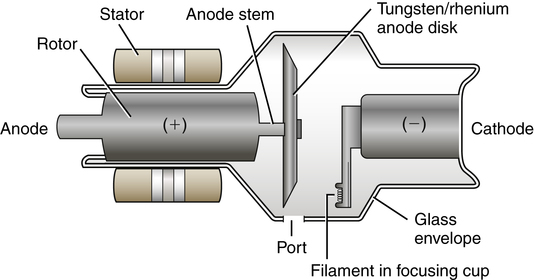
\includegraphics[width=.6\columnwidth,height=4cm]
		{images/xray_tube.jpg}}
	\caption{\label{fig:xrtube} Image of a typical X-Ray tube. The apparatus is enclosed in a vacuum to limit the electrons interactions with air particulates. }
\end{figure}

When the electrons released from the cathode interact with anode material, there is always release of radiation, known as Bremsstrahlung radiation. Depending on the incident angle of the electron and the distance to the atom that it interacts with, varying levels of radiation are given off. This radiation is generated because the incident electron is slowed by the target atomic nucleus, reducing kinetic energy of the incident electron, resulting in the release of radiation. An incident electron can also collide with a target electron, and if the energy exceeds that of the target electron's binding energy, that target electron is ejected. As there is now a vacancy in one of the atoms electron shells, an electron from a lower energy shell will immediately transition to fill it, giving off what is known as characteristic radiation.  Figure \ref{fig:brem} shows a filtered radiation spectrum including the characteristic radiation from an example target material. 


\begin{figure}[H]
	\centerline{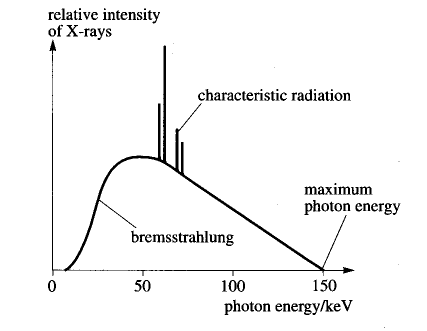
\includegraphics[width=.6\columnwidth,height=4cm] 
		{images/brem.png}}
	\caption{\label{fig:brem} Example radiation spectrum including characteristic radiation. }
\end{figure}